% Options for packages loaded elsewhere
\PassOptionsToPackage{unicode}{hyperref}
\PassOptionsToPackage{hyphens}{url}
\PassOptionsToPackage{dvipsnames,svgnames,x11names}{xcolor}
%
\documentclass[
  12pt,
  letterpaper,
  DIV=11,
  numbers=noendperiod]{scrartcl}

\usepackage{amsmath,amssymb}
\usepackage{iftex}
\ifPDFTeX
  \usepackage[T1]{fontenc}
  \usepackage[utf8]{inputenc}
  \usepackage{textcomp} % provide euro and other symbols
\else % if luatex or xetex
  \usepackage{unicode-math}
  \defaultfontfeatures{Scale=MatchLowercase}
  \defaultfontfeatures[\rmfamily]{Ligatures=TeX,Scale=1}
\fi
\usepackage{lmodern}
\ifPDFTeX\else  
    % xetex/luatex font selection
    \setmainfont[]{Times New Roman}
\fi
% Use upquote if available, for straight quotes in verbatim environments
\IfFileExists{upquote.sty}{\usepackage{upquote}}{}
\IfFileExists{microtype.sty}{% use microtype if available
  \usepackage[]{microtype}
  \UseMicrotypeSet[protrusion]{basicmath} % disable protrusion for tt fonts
}{}
\makeatletter
\@ifundefined{KOMAClassName}{% if non-KOMA class
  \IfFileExists{parskip.sty}{%
    \usepackage{parskip}
  }{% else
    \setlength{\parindent}{0pt}
    \setlength{\parskip}{6pt plus 2pt minus 1pt}}
}{% if KOMA class
  \KOMAoptions{parskip=half}}
\makeatother
\usepackage{xcolor}
\setlength{\emergencystretch}{3em} % prevent overfull lines
\setcounter{secnumdepth}{5}
% Make \paragraph and \subparagraph free-standing
\makeatletter
\ifx\paragraph\undefined\else
  \let\oldparagraph\paragraph
  \renewcommand{\paragraph}{
    \@ifstar
      \xxxParagraphStar
      \xxxParagraphNoStar
  }
  \newcommand{\xxxParagraphStar}[1]{\oldparagraph*{#1}\mbox{}}
  \newcommand{\xxxParagraphNoStar}[1]{\oldparagraph{#1}\mbox{}}
\fi
\ifx\subparagraph\undefined\else
  \let\oldsubparagraph\subparagraph
  \renewcommand{\subparagraph}{
    \@ifstar
      \xxxSubParagraphStar
      \xxxSubParagraphNoStar
  }
  \newcommand{\xxxSubParagraphStar}[1]{\oldsubparagraph*{#1}\mbox{}}
  \newcommand{\xxxSubParagraphNoStar}[1]{\oldsubparagraph{#1}\mbox{}}
\fi
\makeatother


\providecommand{\tightlist}{%
  \setlength{\itemsep}{0pt}\setlength{\parskip}{0pt}}\usepackage{longtable,booktabs,array}
\usepackage{calc} % for calculating minipage widths
% Correct order of tables after \paragraph or \subparagraph
\usepackage{etoolbox}
\makeatletter
\patchcmd\longtable{\par}{\if@noskipsec\mbox{}\fi\par}{}{}
\makeatother
% Allow footnotes in longtable head/foot
\IfFileExists{footnotehyper.sty}{\usepackage{footnotehyper}}{\usepackage{footnote}}
\makesavenoteenv{longtable}
\usepackage{graphicx}
\makeatletter
\def\maxwidth{\ifdim\Gin@nat@width>\linewidth\linewidth\else\Gin@nat@width\fi}
\def\maxheight{\ifdim\Gin@nat@height>\textheight\textheight\else\Gin@nat@height\fi}
\makeatother
% Scale images if necessary, so that they will not overflow the page
% margins by default, and it is still possible to overwrite the defaults
% using explicit options in \includegraphics[width, height, ...]{}
\setkeys{Gin}{width=\maxwidth,height=\maxheight,keepaspectratio}
% Set default figure placement to htbp
\makeatletter
\def\fps@figure{htbp}
\makeatother
% definitions for citeproc citations
\NewDocumentCommand\citeproctext{}{}
\NewDocumentCommand\citeproc{mm}{%
  \begingroup\def\citeproctext{#2}\cite{#1}\endgroup}
\makeatletter
 % allow citations to break across lines
 \let\@cite@ofmt\@firstofone
 % avoid brackets around text for \cite:
 \def\@biblabel#1{}
 \def\@cite#1#2{{#1\if@tempswa , #2\fi}}
\makeatother
\newlength{\cslhangindent}
\setlength{\cslhangindent}{1.5em}
\newlength{\csllabelwidth}
\setlength{\csllabelwidth}{3em}
\newenvironment{CSLReferences}[2] % #1 hanging-indent, #2 entry-spacing
 {\begin{list}{}{%
  \setlength{\itemindent}{0pt}
  \setlength{\leftmargin}{0pt}
  \setlength{\parsep}{0pt}
  % turn on hanging indent if param 1 is 1
  \ifodd #1
   \setlength{\leftmargin}{\cslhangindent}
   \setlength{\itemindent}{-1\cslhangindent}
  \fi
  % set entry spacing
  \setlength{\itemsep}{#2\baselineskip}}}
 {\end{list}}
\usepackage{calc}
\newcommand{\CSLBlock}[1]{\hfill\break\parbox[t]{\linewidth}{\strut\ignorespaces#1\strut}}
\newcommand{\CSLLeftMargin}[1]{\parbox[t]{\csllabelwidth}{\strut#1\strut}}
\newcommand{\CSLRightInline}[1]{\parbox[t]{\linewidth - \csllabelwidth}{\strut#1\strut}}
\newcommand{\CSLIndent}[1]{\hspace{\cslhangindent}#1}

\KOMAoption{captions}{tableheading}
\makeatletter
\@ifpackageloaded{caption}{}{\usepackage{caption}}
\AtBeginDocument{%
\ifdefined\contentsname
  \renewcommand*\contentsname{Table of contents}
\else
  \newcommand\contentsname{Table of contents}
\fi
\ifdefined\listfigurename
  \renewcommand*\listfigurename{List of Figures}
\else
  \newcommand\listfigurename{List of Figures}
\fi
\ifdefined\listtablename
  \renewcommand*\listtablename{List of Tables}
\else
  \newcommand\listtablename{List of Tables}
\fi
\ifdefined\figurename
  \renewcommand*\figurename{Figure}
\else
  \newcommand\figurename{Figure}
\fi
\ifdefined\tablename
  \renewcommand*\tablename{Table}
\else
  \newcommand\tablename{Table}
\fi
}
\@ifpackageloaded{float}{}{\usepackage{float}}
\floatstyle{ruled}
\@ifundefined{c@chapter}{\newfloat{codelisting}{h}{lop}}{\newfloat{codelisting}{h}{lop}[chapter]}
\floatname{codelisting}{Listing}
\newcommand*\listoflistings{\listof{codelisting}{List of Listings}}
\makeatother
\makeatletter
\makeatother
\makeatletter
\@ifpackageloaded{caption}{}{\usepackage{caption}}
\@ifpackageloaded{subcaption}{}{\usepackage{subcaption}}
\makeatother

\ifLuaTeX
  \usepackage{selnolig}  % disable illegal ligatures
\fi
\usepackage{bookmark}

\IfFileExists{xurl.sty}{\usepackage{xurl}}{} % add URL line breaks if available
\urlstyle{same} % disable monospaced font for URLs
\hypersetup{
  pdftitle={Final Report},
  pdfauthor={Dhruv Dole; Nathan Rethwisch; Colin Russell; Thanh Mai},
  colorlinks=true,
  linkcolor={blue},
  filecolor={Maroon},
  citecolor={Blue},
  urlcolor={Blue},
  pdfcreator={LaTeX via pandoc}}


\title{Final Report}
\author{Dhruv Dole \and Nathan Rethwisch \and Colin Russell \and Thanh
Mai}
\date{}

\begin{document}
\maketitle


\section{Introduction/Project
Description}\label{introductionproject-description}

Wildfires are a major problem in the United States, costing between
\$394 billion and \$893 billion per year, according to the Joint
Economic Committee (U.S. Congress Joint Economic Committee 2023).
Identifying where and why wildfires occur is key to preventing
wildfires, which protects lives, preserves property, and minimizes
economic losses. The goal of this project is to estimate areas of high
fire risk based on historical weather patterns and wildfire data. We aim
to provide a platform where users can obtain information about past
weather conditions and their association with wildfires at a quick
glance. This dashboard is designed for a broad audience, including
high-level policymakers involved in wildfire prevention strategies and
local officials responsible for establishing rules and regulations based
on regional wildfire risk.

\begin{figure}[H]

\centering{

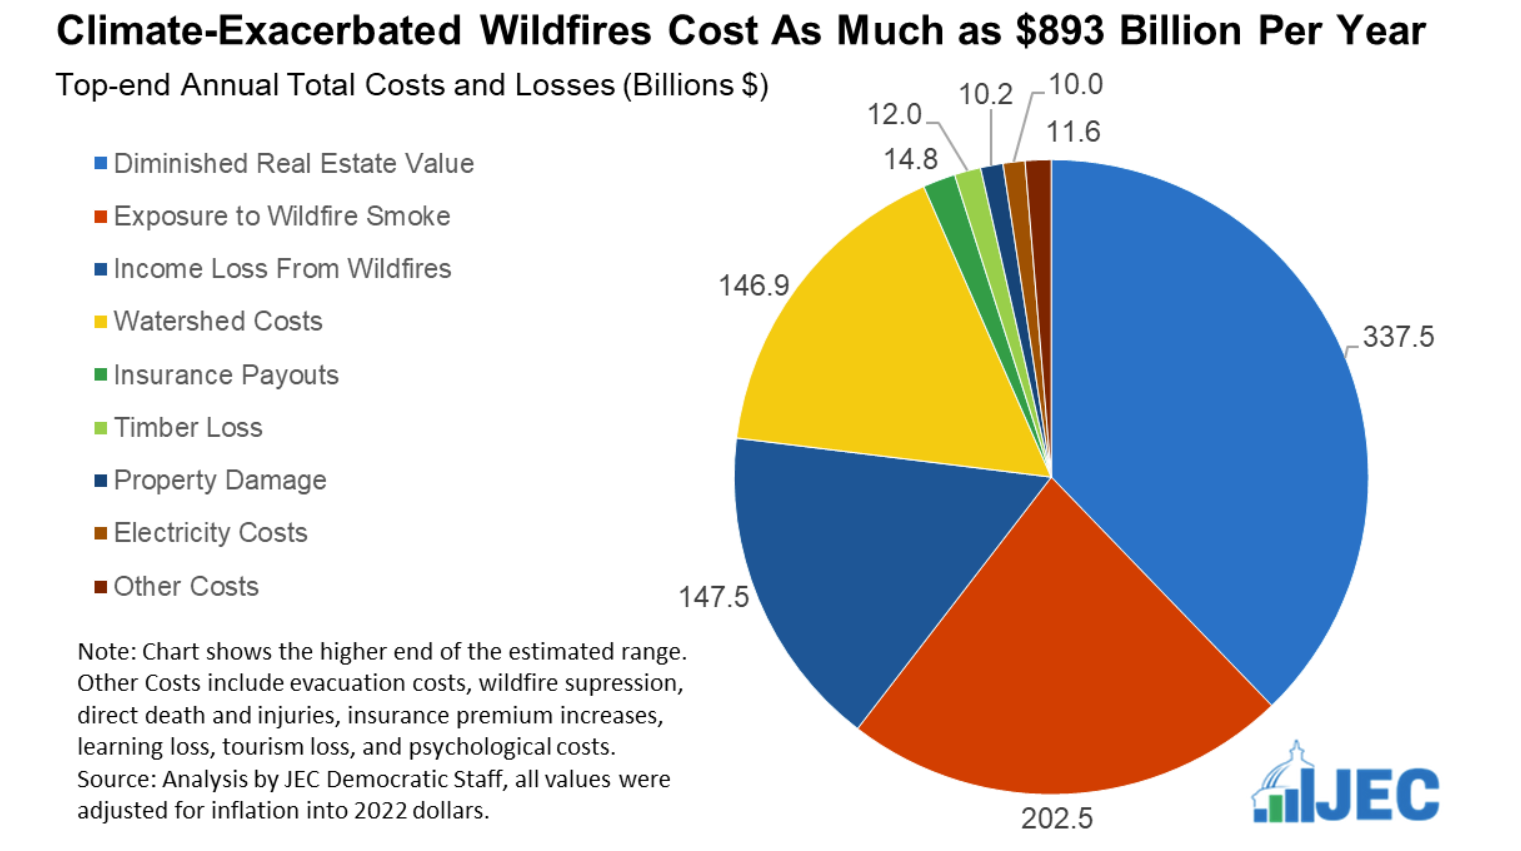
\includegraphics{WildfireCost.png}

}

\caption{\label{fig-WildfireCost}Estimated Cost of Wildfires in 2022}

\end{figure}%

\section{Data Pipeline}\label{data-pipeline}

\subsection{Acquisition}\label{acquisition}

\begin{itemize}
\tightlist
\item
  Description of sources (api, data format)

  \begin{itemize}
  \tightlist
  \item
    GHCN daily (temperature, wind, precipitation, snowfall): Issues with
    lack of documentation, fixed-width files, NOAA servers went down for
    a while in january(politics), A few different available file
    formats, found a public mirror on s3.\\
  \item
    USFS fire perimeter, fire occurrence (coordinates and perimeters of
    each fire incident)\\
  \item
    map polygons and rasters\\
  \item
    other datasets explored but not used: openmeteo api, copernicus
    data, gnatsgo soil data\\
  \end{itemize}
\item
  Acquisitions, rate limits\ldots{}\\
\item
  Process itself
\end{itemize}

\subsection{Transformation}\label{transformation}

The transformations for the GHCN Daily data is a single script because
the required transformations were changing almost every day, and it was
often necessary to rebuild the dataset outright. This also allows for
anyone to reproduce the dataset.

\begin{itemize}
\tightlist
\item
  (TODO: go back to code to get exact steps)\\
\item
  Each transformation applied\\
\item
  Purpose and issues for each major transformation
\end{itemize}

\subsection{Data Cube Storage and
Query}\label{data-cube-storage-and-query}

\begin{itemize}
\tightlist
\item
  Query Requirements and implementation

  \begin{itemize}
  \tightlist
  \item
    Need to run selections, projections, and group by aggregations on a
    larger than memory datasets. (limited by developer hardware).\\
  \item
    Need to be able to query both datatables across the same
    dimensions\\
  \item
    Chose Pyarrow and Parquet as primary system because it allows lazy
    predicate evaluation on larger than memory datasets. Pyarrow
    datasets and tables can be easily converted to pandas dataframes,
    and there is a fully featured Arrow package for R.\\
  \end{itemize}
\item
  Selection and implementation of storage to satisfy said requirements

  \begin{itemize}
  \tightlist
  \item
    Don't want to pay for storage or bandwidth\\
  \item
    Data versioning is unnecessary\\
  \item
    Multiple people need to have concurrent read access, only one person
    will be writing to a table at a time.\\
  \item
    Data is too large for free github LFS\\
  \item
    Dataset is stored in a shared onedrive folder, which is symlinked
    into the local repo by each user. This allows code to use a single
    uniform path, while keeping data access up to the individual
    developer(other developers can download the data to repo/data).
  \end{itemize}
\item
  We assumed needing to have the entire dataset available to the
  dashboard, turns out we only needed the 3-day averages available
  produced for the model output. This allows us to load the dashboard's
  live data into memory on initialization.
\end{itemize}

\section{Exploration and Analysis}\label{exploration-and-analysis}

\begin{figure}[H]

\centering{

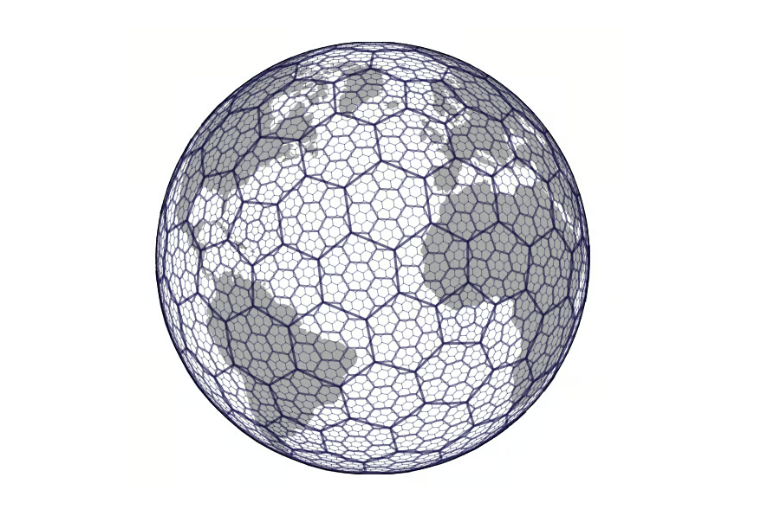
\includegraphics[width=0.5\textwidth,height=\textheight]{UberH3.png}

}

\caption{\label{fig-UberH3}An example of Uber's H3 Cell Grid}

\end{figure}%

After cleaning the data and performing exploratory data analysis, we
realized we needed a way to process data that contained both geospatial
and time information. One additional challenge we faced was the lack of
negative data. Our dataset contained a list of places where fires
occurred, but not where they \emph{did not} occur. Thus, this makes it
difficult to create a binary prediction model of fire probability,
because we only have cases where the fires occurred to train models on.
To solve these problems, we turned to Uber's H3 cell grid, shown in
Figure~\ref{fig-UberH3}. H3 cells are a series of hexagonal cells that
can be used to cover the surface of the globe at different resolutions.
Although perhaps not as precise as certain geographical boundaries for
prediction, H3 hexagons are advantageous because of their computational
speed and equidistant between neighboring cells. In our case, we fit a
grid of cells to the US, with each hexagon representing approximately
4785 square miles, totaling 712 cells. For each day, we marked whether
or not a fire occurred in each hex. Meteorological stations within a
cell were aggregated to compute mean calculations for weather data. The
additional advantage of these cells was that we no longer needed to
spatially join the fire and weather data to perform calculations. Once
we had the index of the cell, we knew exactly which stations were paired
with which fires, saving us the time and computation of continuous
joins.

Another challenge was missing data. If all of the weather stations in a
cell gave null values for a variable on a certain date, they were
imputed with the average from neighboring cells. We also removed
precipitation from our analysis because over 50\% of the precipitation
data was missing.

\section{Modeling}\label{modeling}

\subsection{Data Preparation}\label{data-preparation}

With the addition of H3 cells and negative data for cells without a
fire, we fit a model to predict \(Y_ij\), the probability of a fire
occurring in cell \(i\) on day \(j\), bounded by \([0,1]\). We averaged
the weather variables over three days, the two days before the fire and
the day the fire occurred, for our predictors.\\
Prediction variables were as follows:

\begin{itemize}
\tightlist
\item
  \(x_1\): Hexagon location\\
\item
  \(x_2\): Average Elevation\\
\item
  \(x_3\): Temperature Maximum (3-day average)\\
\item
  \(x_4\): Temperature Minimum (3-day average)\\
\item
  \(x_5\): Daily Average Wind Speed (3-day average)\\
\item
  \(x_6\): Precipitation (3-day average)\\
\item
  \(x_7\): Snowfall (3-day average)\\
\item
  \(x_7\): Month
\end{itemize}

\subsection{Model Selection}\label{model-selection}

We split the data into a training and a testing set. The training data
ranges from January 1, 2000, to December 31, 2019. The testing data was
from January 1, 2020, to March 23, 2025. I encoded the hexagonal
location as numeric variables and ran 4 separate models: logistic
regression, random forest, XGBoost, and Naive Bayes. After running the
models, I then simulated thresholds from 0-1 at a 0.01 interval and
selected the optimal prediction threshold for each model that maximized
the F1 score, which can be defined as
\(\frac{\text{precision} \cdot \text{recall}}{\text{precision} + \text{recall}}\).

\begin{itemize}
\tightlist
\item
  Precision is defined as how often a positive wildfire prediction is
  correctly positive. It can be defined as
  \(\frac{\text{TP}}{\text{TP} + \text{FP}}\).\\
\item
  Recall describes the rate at which the model can correctly identify
  true positives from all possible values. It can be defined as
  \(\frac{\text{TP}}{\text{TP} + \text{FN}}\).
\end{itemize}

F1 score is preferential to accuracy in this case, because the dataset
is imbalanced and we have very few actual positive cases of wildfires,
so models that maximize accuracy are likely to underestimate the
probability of a fire occurring, a more costly mistake than a false
positive.

Figure~\ref{fig-thresholds} shows the optimal thresholds curves, while
Figure~\ref{fig-modelTable} displays statistics for each model in the
selection process.

\begin{figure}[H]

\centering{

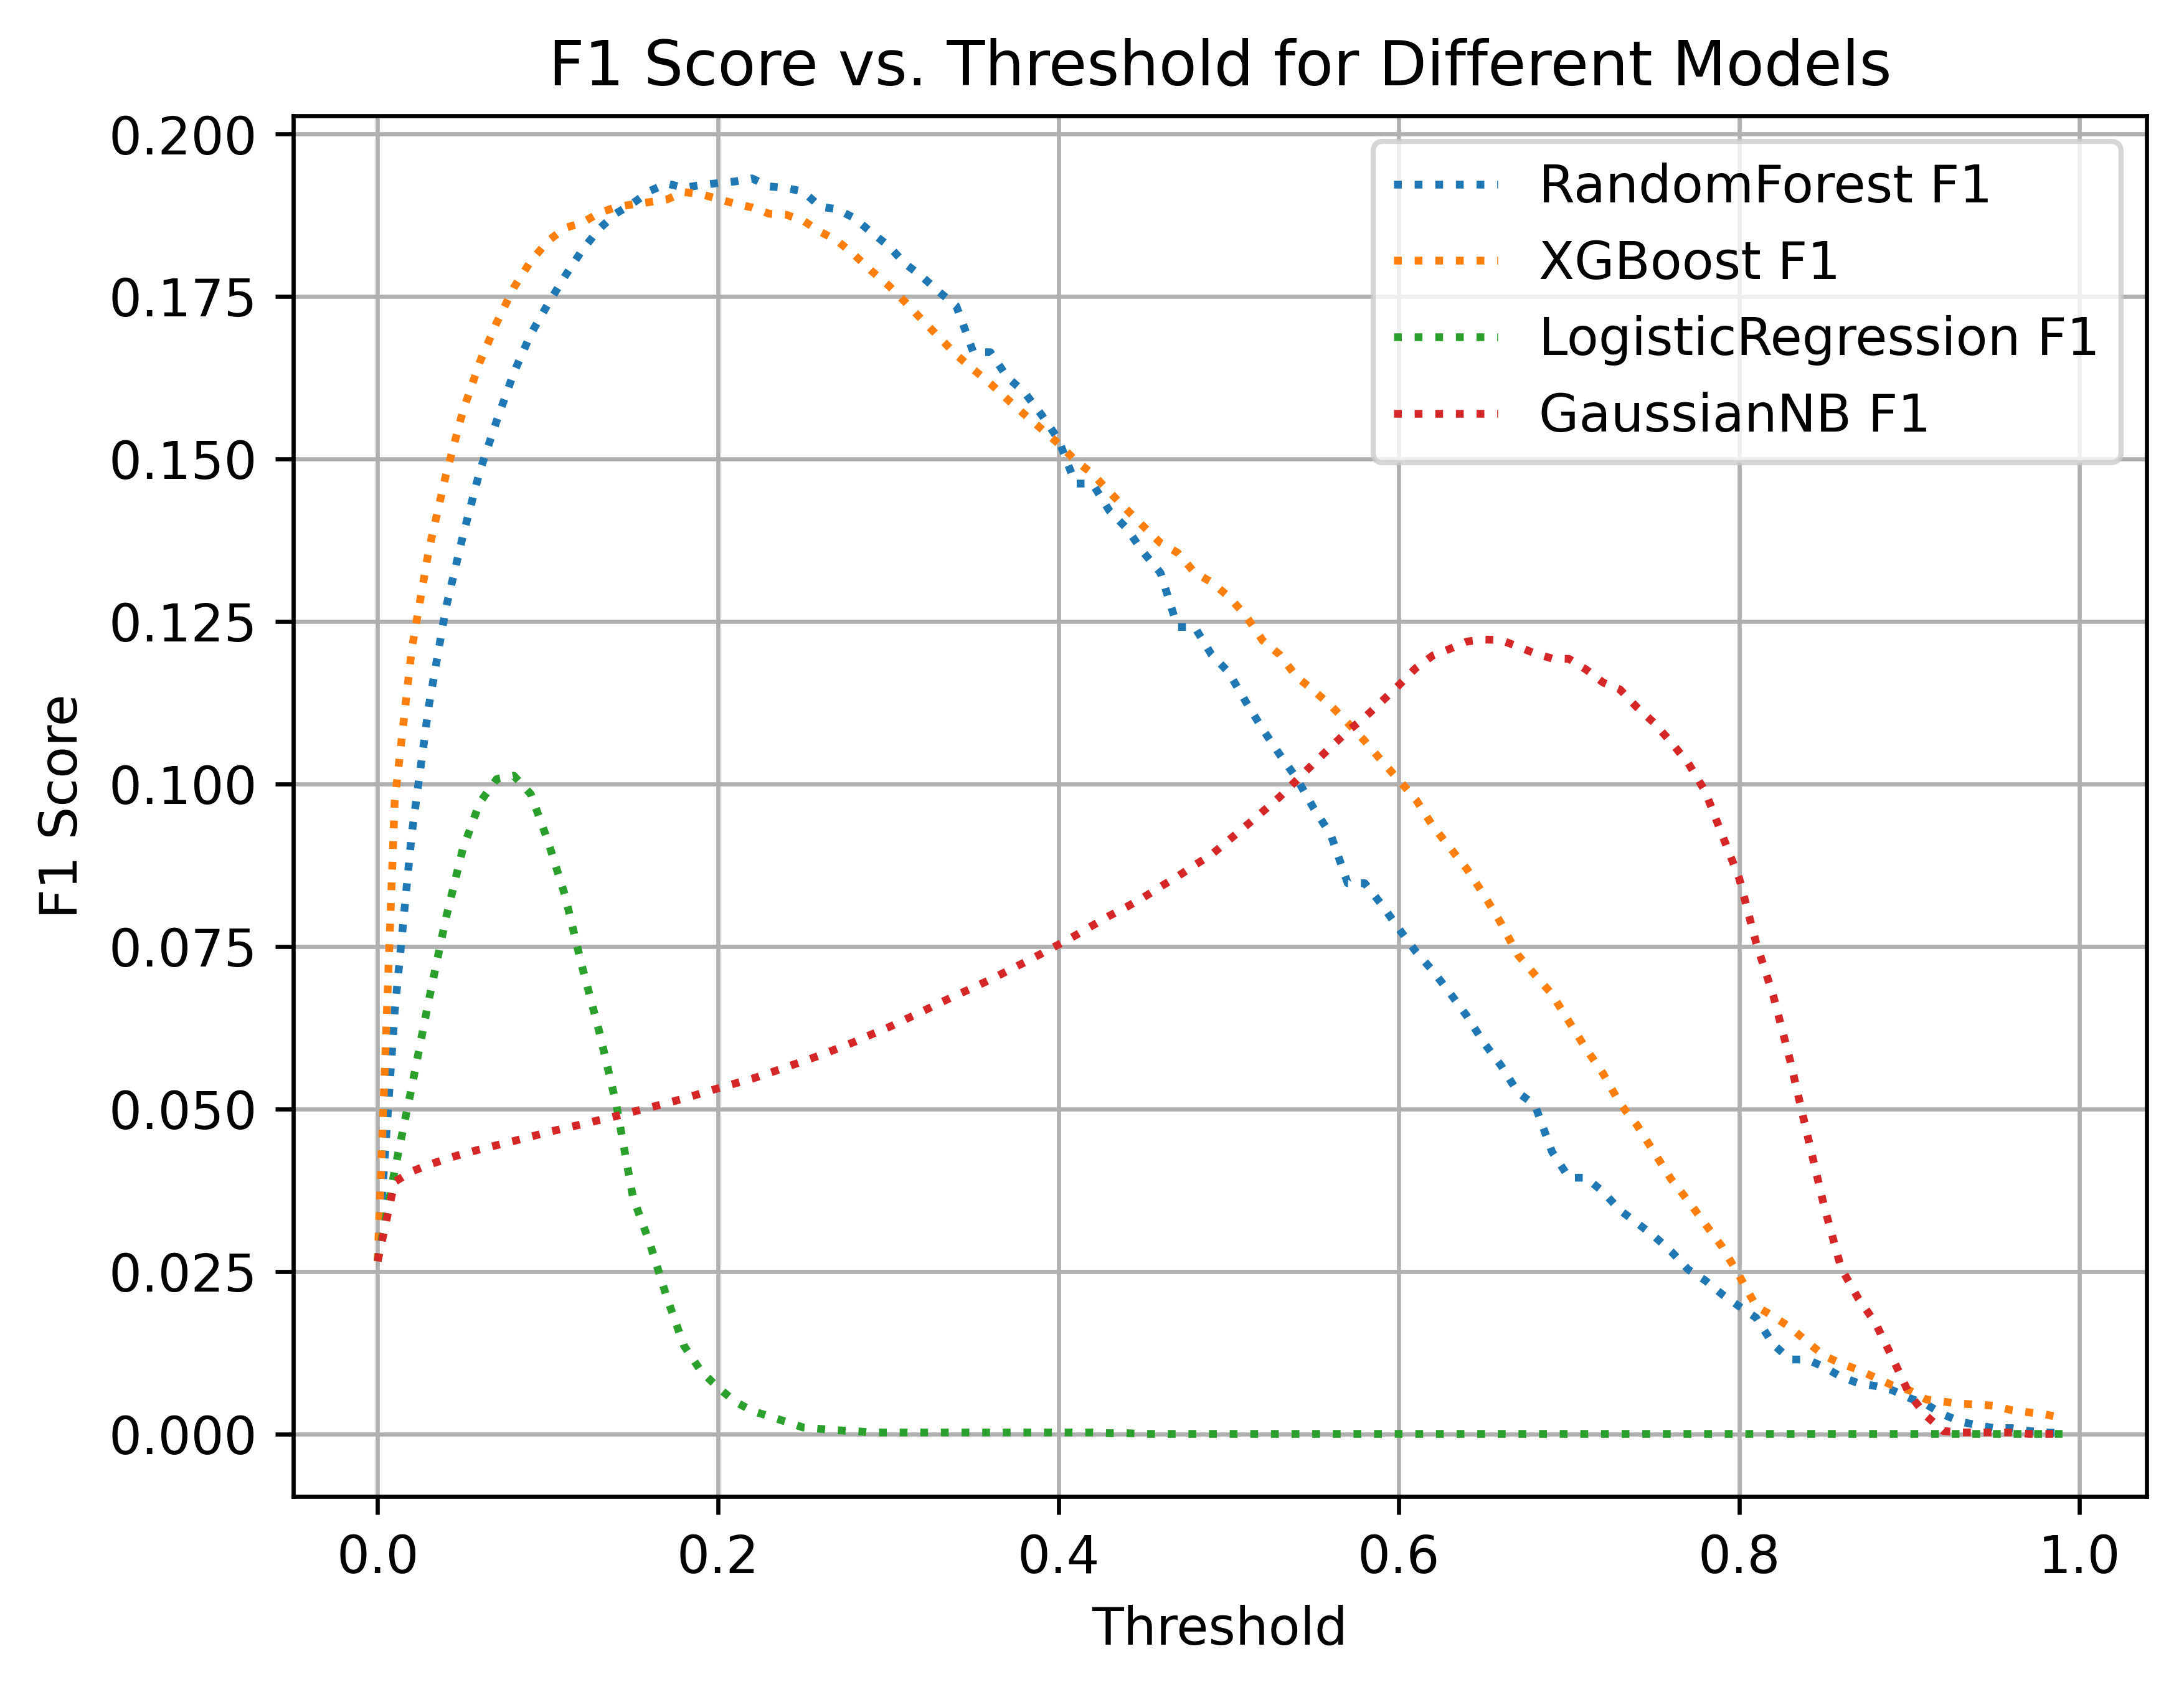
\includegraphics[width=0.5\textwidth,height=0.5\textheight]{thresholds.png}

}

\caption{\label{fig-thresholds}Thresholds for the optimal F1 score using
each model}

\end{figure}%

\begin{figure}[H]

\caption{\label{fig-modelTable}Statistics for each model fit on
historical weather data}

\centering{

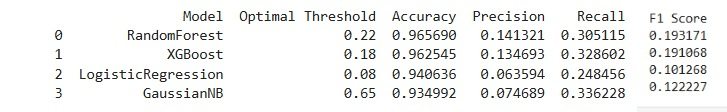
\includegraphics{modelStats.jpg}

}

\end{figure}%

Based on these results, we decided to go with a random forest model.
Although the XGBoost and random forest models performed similarly, the
random forest model had a higher F1 score as well as higher accuracy.
Furthermore, we are more familiar with working with random forests.
Given more time, we would explore the XGBoost model, especially since it
has higher recall, which is desirable given that the cost of a false
negative is high.

\subsection{Hyperparameter Selection}\label{hyperparameter-selection}

After deciding on a random forest as the optimal model, we performed a
grid search with 3-fold cross-validation to fine-tune model parameters.
We used a random sample of 10\% of the data due to storage limits. The
parameters of interest were the number of estimators in the forest (50,
100, 200), the maximum depth of each tree considered (None, 10, 20, 30),
and the number of features considered at each split (2, 3). Therefore,
24 possible combinations were considered. Using a decision threshold of
0.22, we selected the model with the highest F1 score. Ultimately, this
was selected to be one with 200 estimators, a max depth of 30, and 3
features considered at each split. Figure~\ref{fig-codeRF} shows the
trained random forest using this

\begin{figure}[H]

\centering{

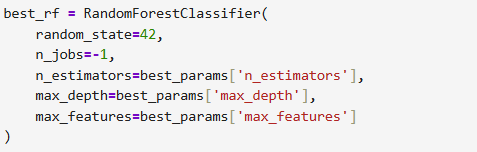
\includegraphics{BestRandomForest.png}

}

\caption{\label{fig-codeRF}Code for Training the Optimal Random Forest}

\end{figure}%

\subsection{Results}\label{results}

After fitting the fine-tuned model to the training and testing data, we
ended with Figure~\ref{fig-bestModelStats}. Hyperparameter tuning was
able to marginally improve F1 score (0.193 to 0.197) and recall (0.305
to 0.330). Although these scores are still fairly low, this is somewhat
expected due to the limit of our data and the variability of fire
causes. Figure~\ref{fig-featureImportance} shows a table of the most
important features, showing that location, elevation, and temperature
were seen as key predictors of wildfires.

\begin{figure}[H]

\caption{\label{fig-bestModelStats}Statistics for our Random Forest
after Hyperpararmeter Tuning}

\centering{

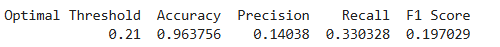
\includegraphics{bestModelStats.png}

}

\end{figure}%

\begin{figure}[H]

\caption{\label{fig-featureImportance}Feature Importance}

\centering{

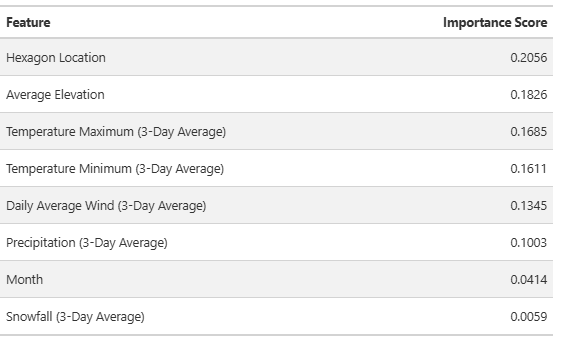
\includegraphics[width=0.7\textwidth,height=0.7\textheight]{featureImportance.png}

}

\end{figure}%

After running the model, the output was saved as a parquet file and
loaded later into the dashboard.

\subsection{Challenges}\label{challenges}

One of the key challenges faced when running the model was the large
amount of data we faced. Because we are dealing with both time and
spatial data, we were dealing with a dataframe that has a row for every
unique combination of dates from 2020-2025 and hexagon locations (of
which there are 712). This gives a dataset with a total of 188,240,121
rows. This was too large to load into memory on our local devices, so we
used The Catalyst. This is a high-performance computer that is
reservable for students at the Iowa State Library. We loaded the data
and were able to save the model output through OneDrive.

\section{Dashboard}\label{dashboard}

\subsection{Exploration}\label{exploration}

We originally explored ArcGIS's online dashboarding tools due to its
seamless integration with geospatial data. However, loading hexagonal
maps with predictions for each date proved to be too large a task for
the software to handle, leading to incredible slow loading times. As a
result, we turned to Python's Dash library. This was able to handle
large amounts of data and gave the option to add map layers easily.

\subsection{Dashboard Creation}\label{dashboard-creation}

\begin{itemize}
\tightlist
\item
  Explored arcgis(slow, generally too limited in feature set)\\
\item
  Chose dash because data was large and required cu\\
\item
  stom real-time querying, needed efficient real-time map generation and
  rendering\\
\item
  Stack: mixed python/r, dash, leaflet, containerized with docker,
  self-hosted\\
\item
  Key visualization: fire risk probability, climate data\\
\item
  Precomputed all values and plots needed for dashboard. The only
  realtime workload is selecting a single day's render fields.\\
\item
  many many pictures
\end{itemize}

All of the values for the dashboard were precomputed from the model. For
the colors of the map, output was normalized using the following
formula:\\
\[\frac{x - x_{min}}{x_{max} - x_{min}}\]\\
However, the actual predicted output and color bar on the map reverse
this normalization so that the labels match the real predicted and
weather values.

\subsection{Interface}\label{interface}

The dashboard has three main tabs. The map view allows users to set a
date to view an overlay of wildfire predictions within hexagons on a map
of the United States. The user can select the date displayed using a
date slider at the bottom of the page. They can also select different
variables in the tab menu on the map to get weather data for that date,
allowing users to easily visualize weather patterns and areas of high
fire probability. When viewing the map, users can click on a specific
hex to get both model output and weather for that area on that selected
date. Model output can be copied to clipboard for advanced analytics and
reporting.

The time series plot was created in Python using Plotly and is hosted as
an HTML file. This gives information on the number of fires occurring on
a weekly, monthly, and yearly basis.

Finally, the dashboard info tab gives information about the underlying
model and how to use the dashboard. It was created in R using Quarto and
is also implemented as an HTML.

\begin{figure}[H]

\centering{

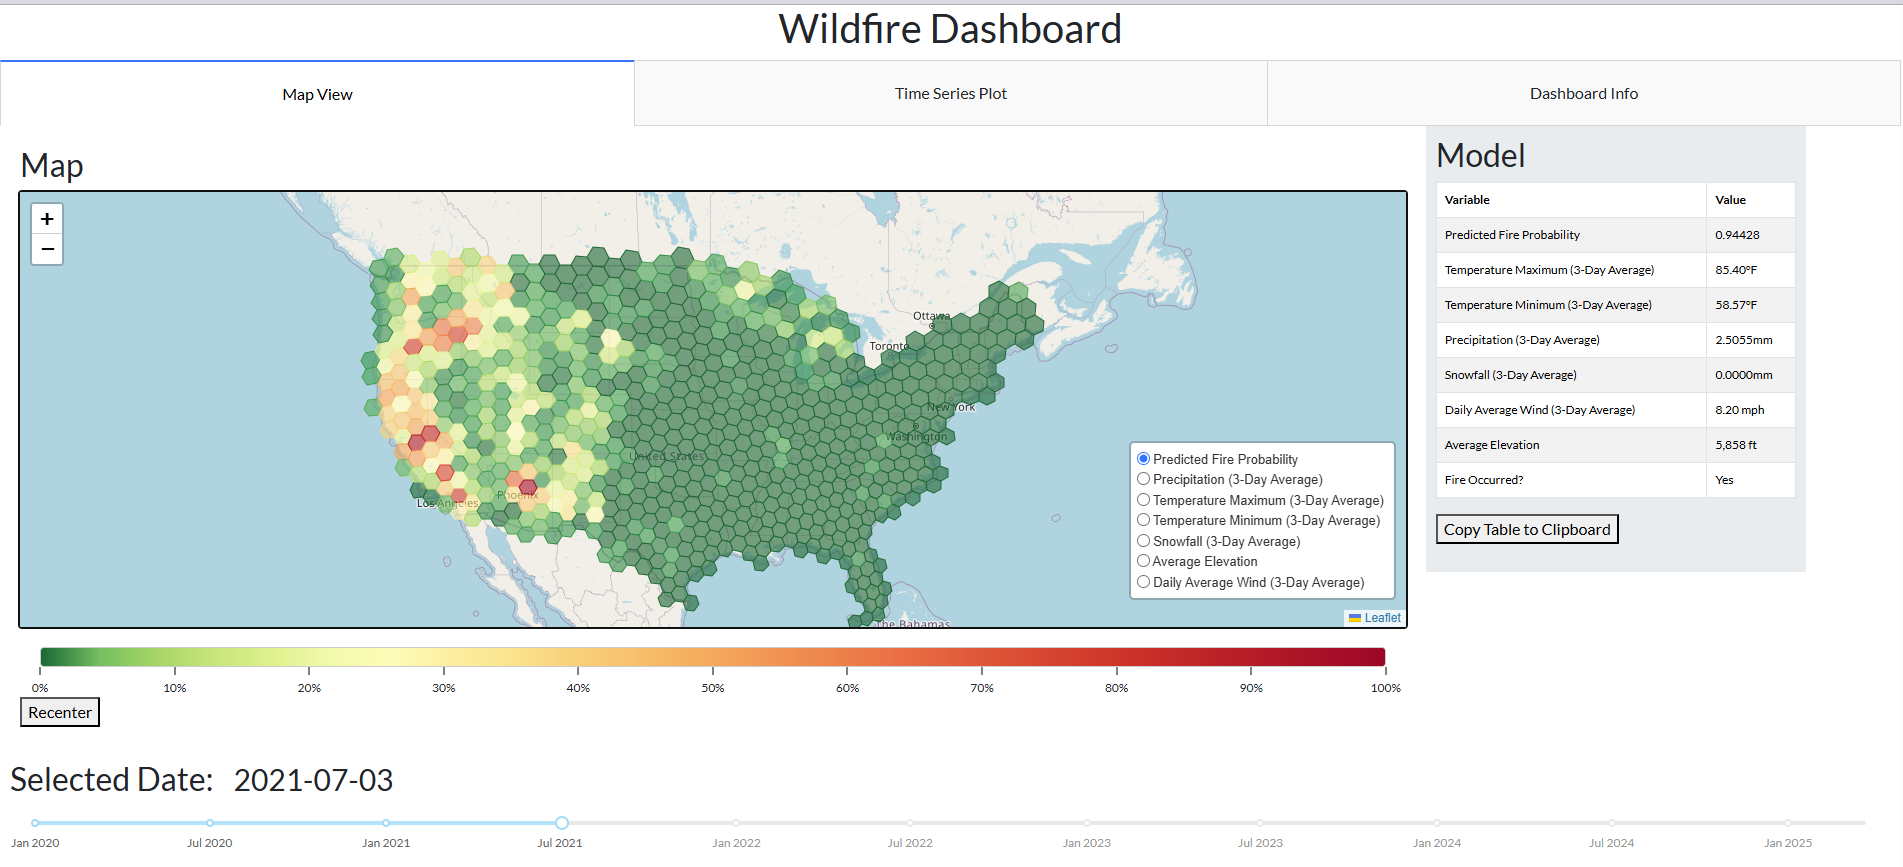
\includegraphics{dashboard.png}

}

\caption{\label{fig-dashboard}An example wildfire prediction dashboard}

\end{figure}%

\subsection{Challenges}\label{challenges-1}

\begin{itemize}
\tightlist
\item
  Major issues and solutions (dash-leaflet immutability)
\end{itemize}

\subsection{Availability/Source Code
Location}\label{availabilitysource-code-location}

All of the source code can be found at
\url{https://github.com/nathanrethwisch/FinalProjectDS4010A}. The
dashboard is currently hosted at \url{https://wildfire.ddole.net/}.

\section{Conclusion}\label{conclusion}

\subsection{Summary}\label{summary}

Using historical fire data from the United States Forest Service (USFS)
and weather data from the National Oceanic and Atmospheric
Administration (NOAA), we were able to create a random forest model and
associated dashboard that predicted the probability of a fire occurring
in a given area on a certain date. The dashboard allows users to explore
dates and weather trends that lead to a high fire probability. This can
be used for setting policy and garnering a greater understanding of the
relationship between weather and wildfires.

\subsection{Further Discussion}\label{further-discussion}

Given more time, we would aim to expand our analysis by incorporating
additional datasets to enhance our predictive accuracy. We would include
factors such as soil conditions and wind direction in specific areas as
key predictors. Additionally, we would like to explore the probability
of a fire occurring again in a region that has already had a recent
wildfire. If we had access to greater computational resources, we would
refine our predictions by using smaller hexagonal grids, allowing for
more precise insights into distinct geographical climates. Moreover, the
dashboard could be enhanced to support future fire prediction efforts.
By using upcoming weather forecasts, we could provide a forecasted
probability of fire occurrence in specific areas. These ideas lay the
foundation for ongoing exploration and continued development of the
dashboard.

\subsection*{Sources}\label{sources}
\addcontentsline{toc}{subsection}{Sources}

\phantomsection\label{refs}
\begin{CSLReferences}{1}{0}
\bibitem[\citeproctext]{ref-jec2023wildfires}
U.S. Congress Joint Economic Committee. 2023. {``Climate-Exacerbated
Wildfires Cost the u.s. Between \$394 to \$893 Billion Each Year in
Economic Costs and Damages.''}
\url{https://www.jec.senate.gov/public/_cache/files/9220abde-7b60-4d05-ba0a-8cc20df44c7d/jec-report-on-total-costs-of-wildfires.pdf}.

\end{CSLReferences}




\end{document}
